\documentclass{beamer}
\usetheme{metropolis}           % Use metropolis theme

\usepackage{tikz}
\usepackage[utf8]{inputenc}
\usepackage[spanish]{babel}

\usepackage{smartdiagram}
\usepackage{qtree}
\usepackage{verbatim}
\usepackage{svg}
\usepackage{graphicx}
\usepackage{color}
\definecolor{lightgray}{rgb}{0.95, 0.95, 0.95}
\definecolor{darkgray}{rgb}{0.4, 0.4, 0.4}
%\definecolor{purple}{rgb}{0.65, 0.12, 0.82}
\definecolor{editorGray}{rgb}{0.95, 0.95, 0.95}
\definecolor{editorOcher}{rgb}{1, 0.5, 0} % #FF7F00 -> rgb(239, 169, 0)
\definecolor{editorGreen}{rgb}{0, 0.5, 0} % #007C00 -> rgb(0, 124, 0)
\definecolor{orange}{rgb}{1,0.45,0.13}		
\definecolor{olive}{rgb}{0.17,0.59,0.20}
\definecolor{brown}{rgb}{0.69,0.31,0.31}
\definecolor{purple}{rgb}{0.38,0.18,0.81}
\definecolor{lightblue}{rgb}{0.1,0.57,0.7}
\definecolor{lightred}{rgb}{1,0.4,0.5}
\usepackage{upquote}
\usepackage{listings}
\lstset{language=html,
	basicstyle=\footnotesize\ttfamily,
	keywordstyle=\footnotesize\color{blue}\ttfamily,
}

\usebackgroundtemplate%
{%
	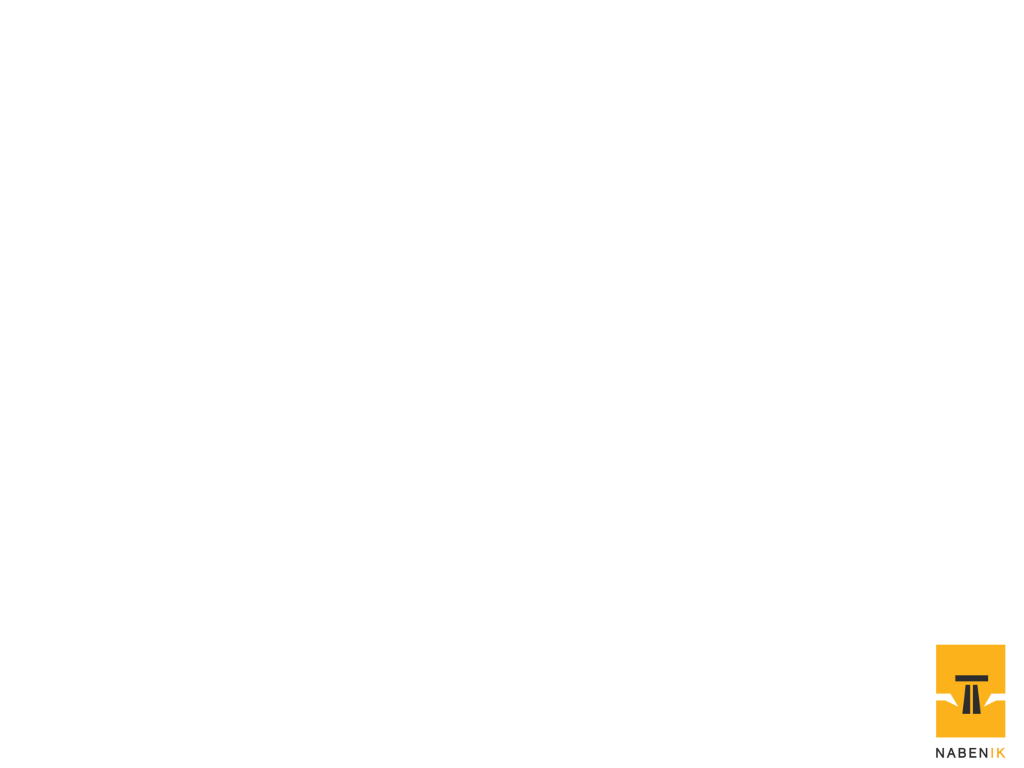
\includegraphics[width=\paperwidth]{Images/fondo}%
}

\title{Microservicios con JavaEE}
\author{Víctor Orozco - @tuxtor}
\institute{GuateJUG}
\date{\today}

\begin{document}

\frame{\titlepage}

\begin{frame}{Acerca de}
\begin{columns}[T] % contents are top vertically aligned
	\begin{column}[T]{5cm} % each column can also be its own environment
		\begin{itemize}
			\item Developer (JVM/Open Source Advocate)
			\item Consultor independiente (Nabenik)
			\item \href{https://twitter.com/tuxtor}{GuateJUG}
			\item \href{https://twitter.com/tuxtor}{@tuxtor}
			\item \href{http://vorozco.com}{The J*} 
		\end{itemize}
	\end{column}
	\begin{column}[T]{5cm} % alternative top-align that's better for graphics
		\begin{figure}
			\centering
			
\includegraphics[width=0.7\linewidth]{Images/logos}
		\end{figure}
		
	\end{column}
\end{columns}
\end{frame}

\section{J2EE}

\begin{frame}{J2EE}
\begin{figure}
	\centering
	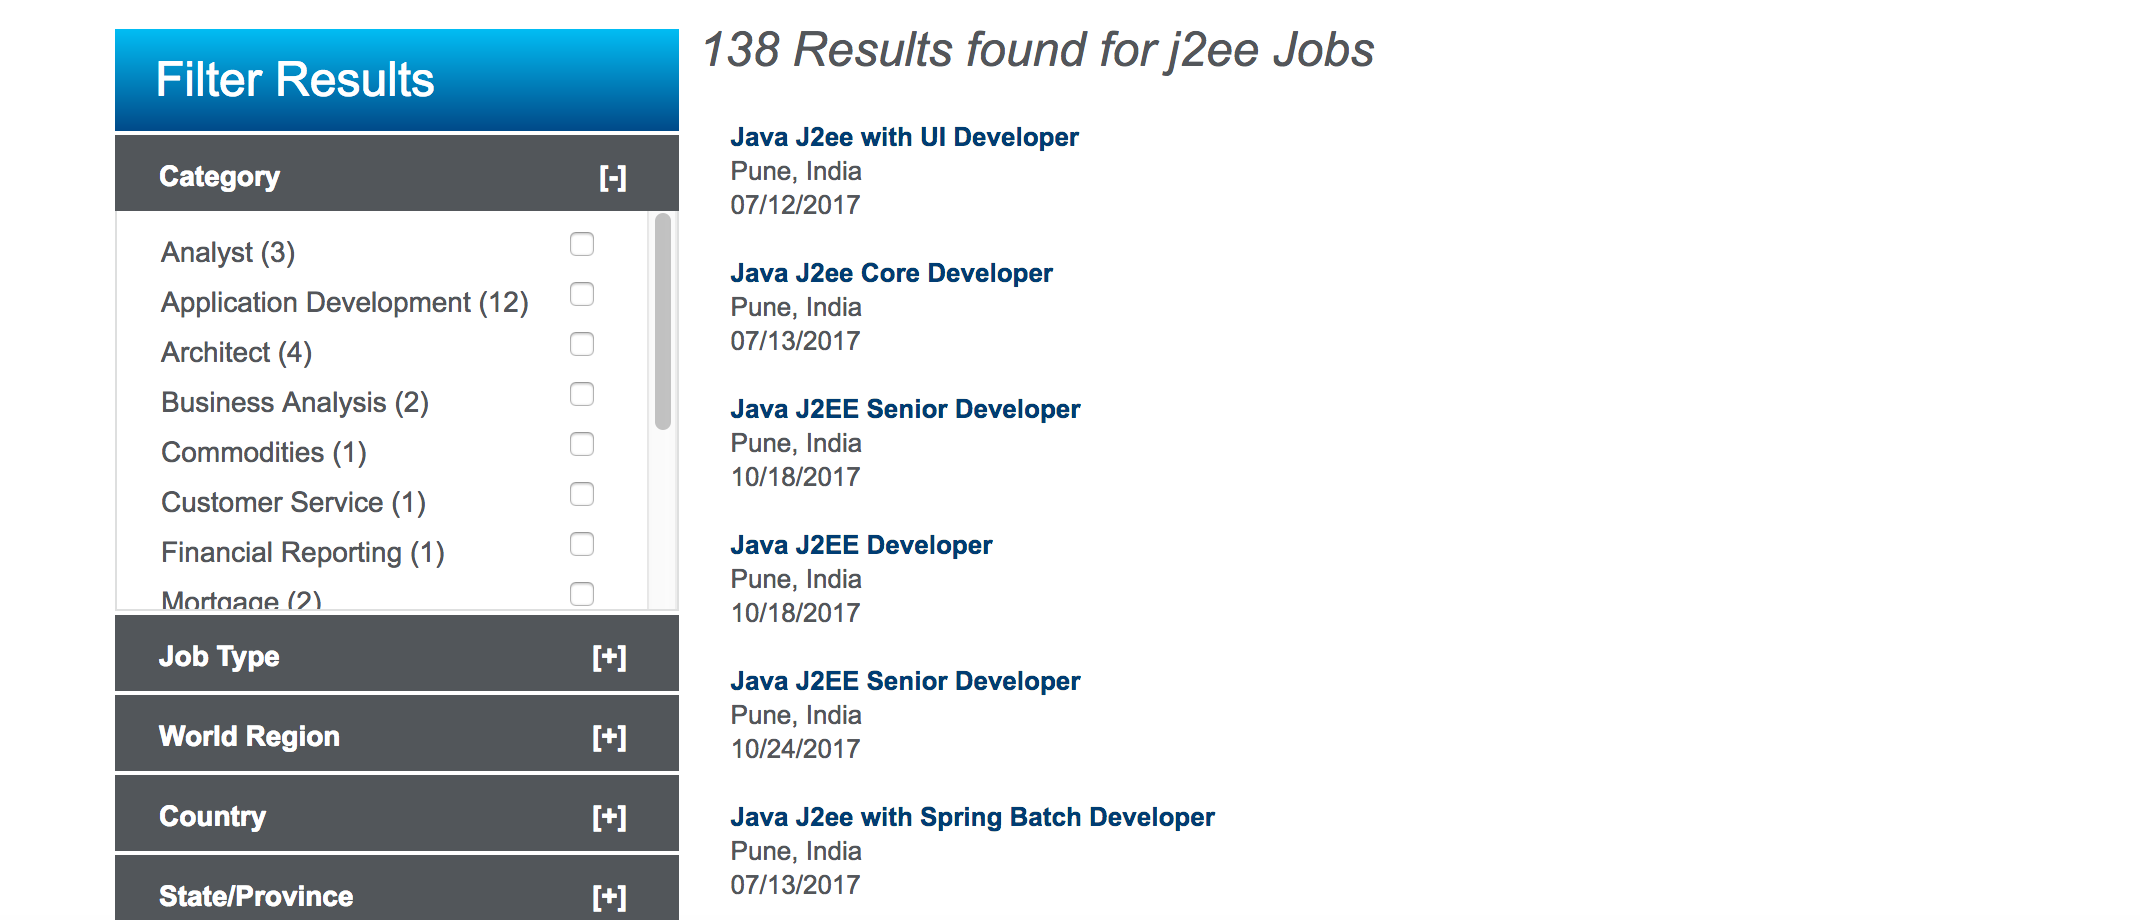
\includegraphics[width=\linewidth]{Images/jobs}
\end{figure}
\end{frame}

\begin{frame}{J2EE}
\begin{figure}
	\centering
	
\includegraphics[width=0.6\linewidth]{Images/futuro}
\end{figure}
\end{frame}

\section{Java EE 7}

\begin{frame}{JavaEE 7}
\begin{figure}
	\centering
	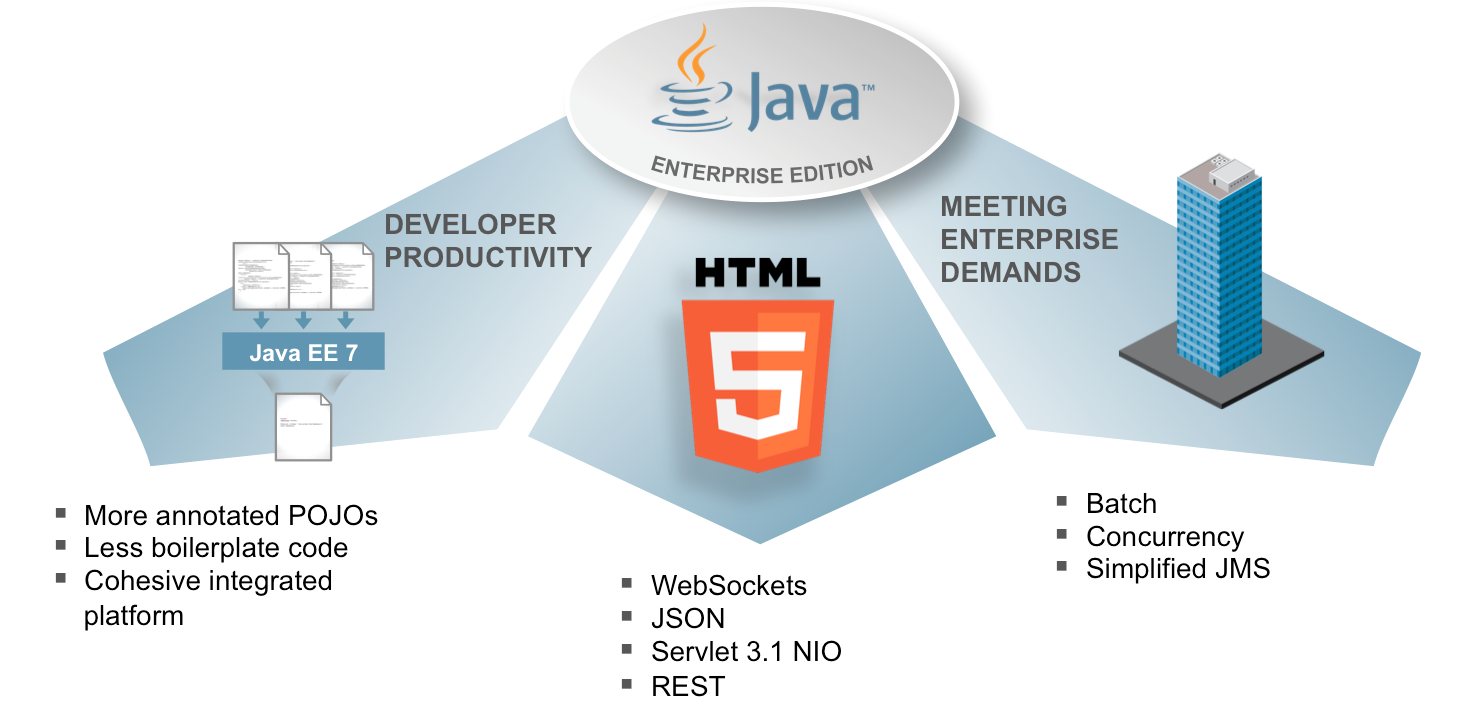
\includegraphics[width=0.75\linewidth]{Images/javaee7-theme}
\end{figure}
\end{frame}

\begin{frame}{JavaEE 7}
\begin{exampleblock}{JavaEE 7}
	\begin{itemize}
		\item Nuevo JMS
		\item WebSockets
		\item JSON Support
		\item Concurrency
		\item Nuevo JAX-RS
		\item Batch apps
	\end{itemize}
\end{exampleblock}
\end{frame}



\section{Java EE 7 - La rebelión de los Dukes}

\begin{frame}{JavaEE 7 - La rebelión}
\begin{columns}
	\begin{column}{0.5\textwidth}
		\begin{figure}
			\centering
			
\includegraphics[width=\linewidth]{Images/microprofile-logo}
		\end{figure}
	\end{column}
	\begin{column}{0.5\textwidth}  %%<--- here
		\begin{figure}
			\centering
			
\includegraphics[width=\linewidth]{Images/guardians}
		\end{figure}
	\end{column}
\end{columns}
\end{frame}

\section{JavaEE Micro}

\begin{frame}{Solución}
Estado zen del arquitecto de software
\begin{itemize}
	\item \textbf{Productividad} - Java 8
	\item Recurso humano - POO -> Funcional
	\item \textbf{¿Predictibilidad y estabilidad?}
	\item \textbf{¿Escalabilidad?}
	\begin{itemize}
		\item \textbf{App Server} - Vertical y luego horizontal
		\item \textbf{Microservicios} - Horizontal
	\end{itemize}
	\item Costos - Todas las anteriores
\end{itemize}
\end{frame}

\begin{frame}{Solución}
\begin{figure}
	\centering
	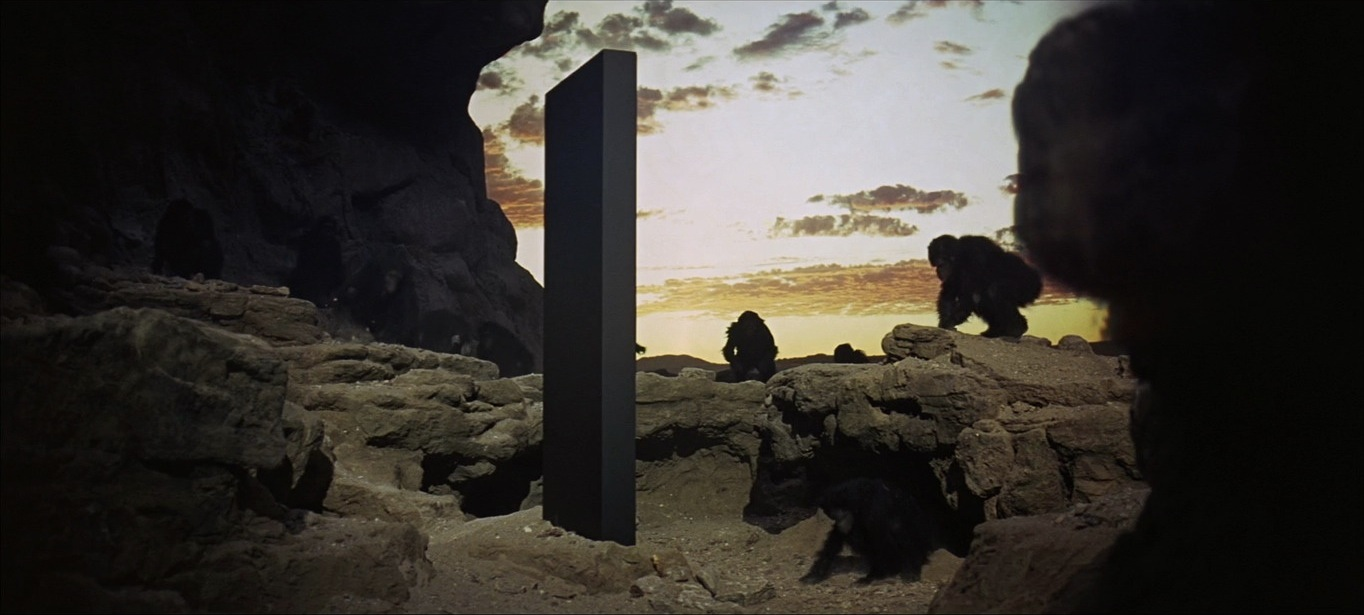
\includegraphics[width=\linewidth]{Images/monolith}
\end{figure}
\end{frame}

\begin{frame}{Monolito}
\begin{figure}
	\centering
	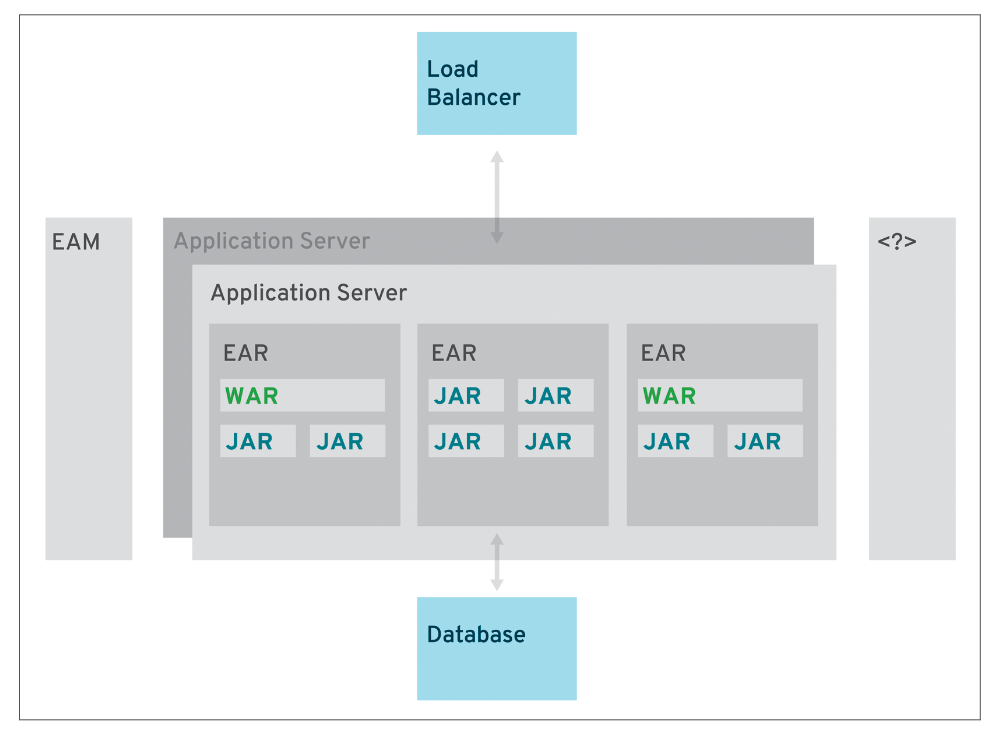
\includegraphics[width=0.7\linewidth]{Images/monolitos}
	\caption{Arquitectura monolitica - Creditos: Markus Eisele}
\end{figure}
\end{frame}

\begin{frame}{ESB}
\begin{figure}
	\centering
	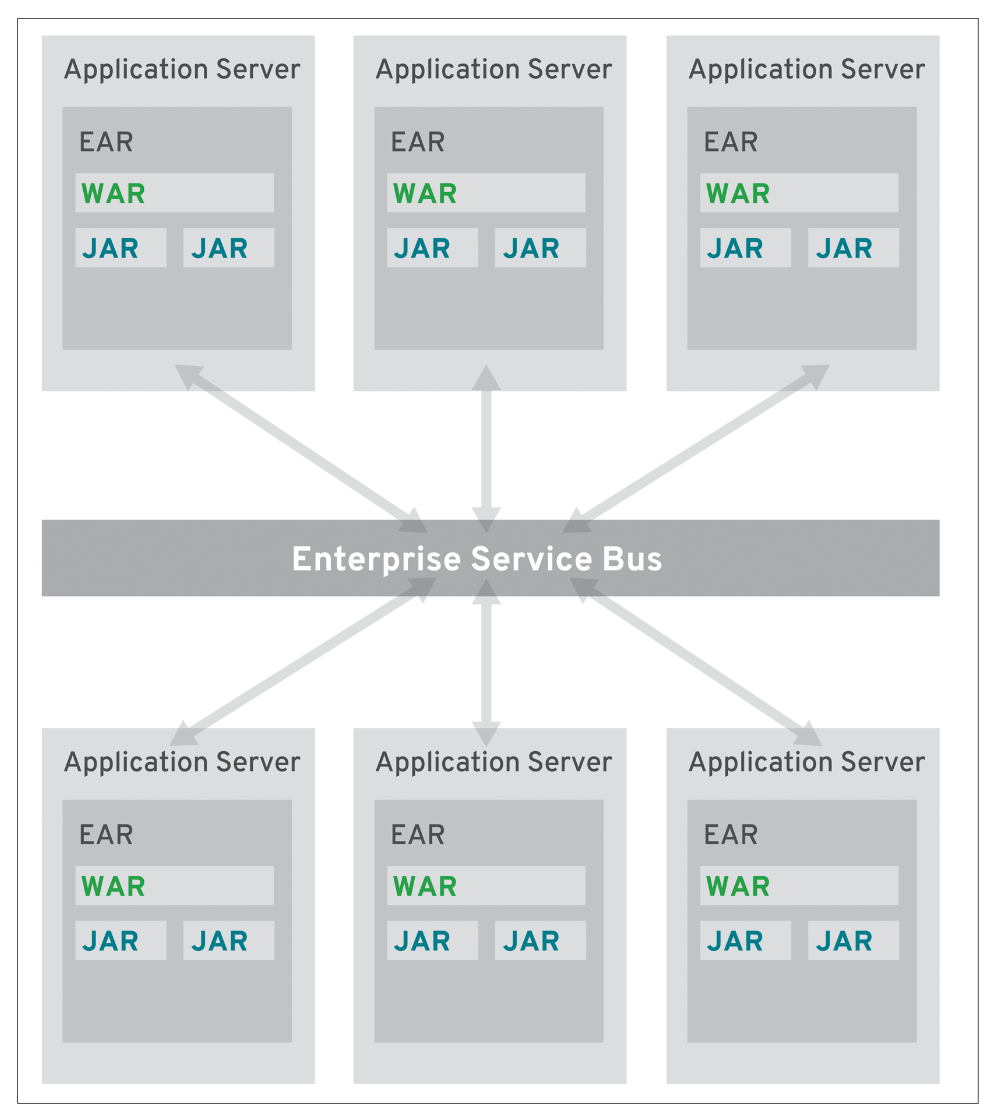
\includegraphics[width=0.5\linewidth]{Images/esb}
	\caption{Arquitectura Esb - Creditos: Markus Eisele}
\end{figure}
\end{frame}

\begin{frame}{Microservicios}
\begin{figure}
	\centering
	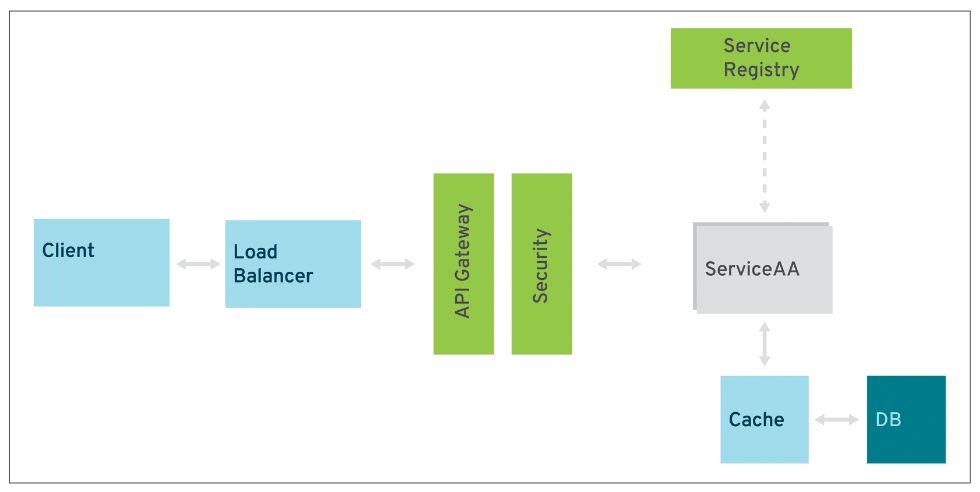
\includegraphics[width=\linewidth]{Images/microservicios}
	\caption{Arquitectura Microservicio - Creditos: Markus Eisele}
\end{figure}
\end{frame}



\begin{frame}{Microservicios}
Ventajas
\begin{itemize}
	\item Bases de código pequeñas
	\item Buenas practicas de programación
	\item Tolerancia a fallas
	\item Escalabilidad
\end{itemize}
Desventajas
\begin{itemize}
	\item Tooling overhead
	\item Debug
	\item Transacciones distribuidas
	\item Latencia
	\item Interdependencia
		\item Falacias de la computación distribuida
\end{itemize}
\end{frame}


\begin{frame}{Microservicios}
Desventaja \\

\huge Hype Driven Development
\end{frame}

\section{Microservicios funcionales con JavaEE}
\begin{frame}{Microservicios - JavaEE}
JavaEE el framework más anti-hype de la tierra\\

\huge J2EE 1.2 (Diciembre 12, 1999)
\end{frame}


\begin{frame}{Microservicios - JavaEE}
Implementación
\begin{itemize}
	\item Refactoring iterativo
	\item Refactoring practico
	\item Nuevos servicios
\end{itemize}
\end{frame}

\begin{frame}{Microservicios - JavaEE}
Implementación
\begin{itemize}
	\item \textbf{Refactoring iterativo}
	\item \textbf{Refactoring practico}
	\item \textbf{Nuevos servicios}
\end{itemize}
\end{frame}

\begin{frame}{Microservicios - JavaEE}
Subset de Api en JavaEE
\begin{itemize}
	\item JAX-RS
	\item JSON-P
	\item CDI, EJB
	\item JCache, JPA
\end{itemize}

Nuevas formas de despliegue
\begin{itemize}
	\item Versiones micro JavaEE (CLI)
	\item Uber-Jar/Fat-Jar
\end{itemize}
\end{frame}

\begin{frame}{Microservicios - JavaEE}
Opciones
\begin{itemize}
	\item \textbf{Wildfly Swarm}
	\item KumuluzEE
	\item Dropwizard
	\item WebSphere Liberty
	\item \textbf{Payara Micro}
\end{itemize}

\end{frame}

\section{Demo}
\begin{frame}{JavaEE Micro  - Demo}
\huge Java 8, JAX-RS, CDI, EJB, JCache

\normalsize  \url{https://github.com/tuxtor/javaee-hol}
\end{frame}

\begin{frame}{Payara Micro - Demo}
\begin{figure}
	\centering
	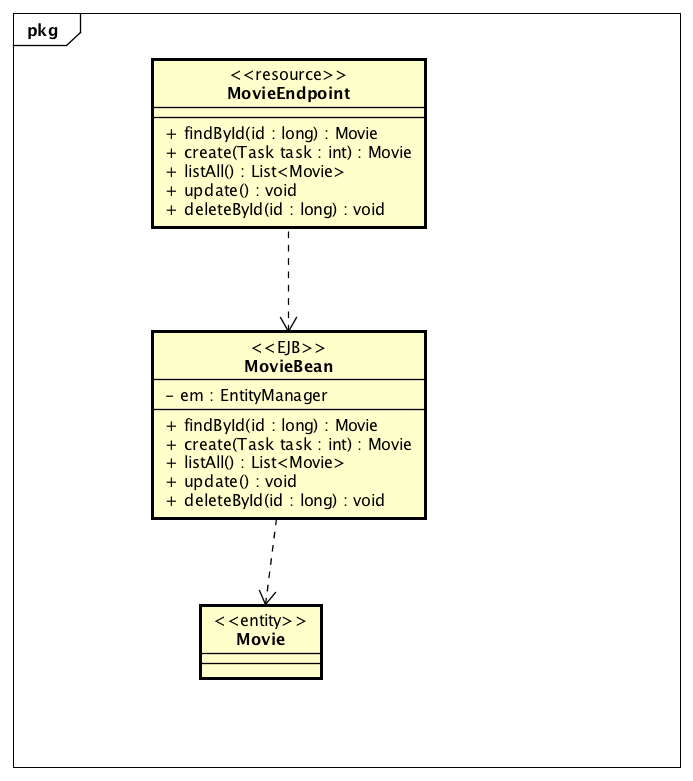
\includegraphics[width=0.6\linewidth]{Images/democlass}
\end{figure}
\end{frame}

\section{Java EE 8}
\begin{frame}{JavaEE 8}
\begin{figure}
	\centering
	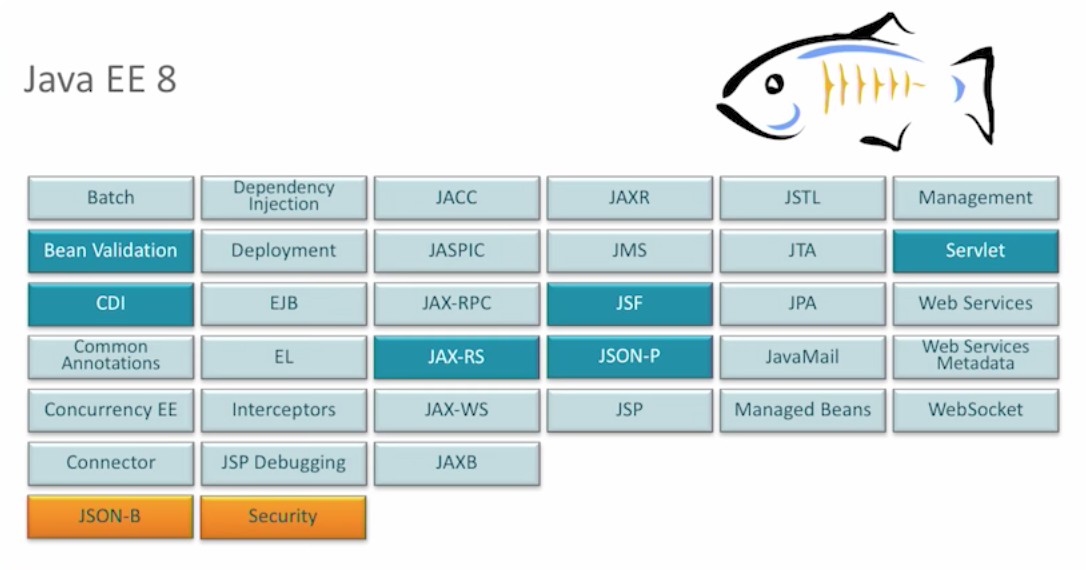
\includegraphics[width=0.9\linewidth]{Images/javaee8}
\end{figure}
\end{frame}


\begin{frame}{JavaEE 8}
\begin{alertblock}{JavaEE 8}
	\begin{itemize}
		\item Mejor integración de JSF con CDI
		\item Mejor integración de JMS con CDI
		\item HTTP/2
		\item JSON-B
		\item Security
		\item JAX-RS Reactivo
	\end{itemize}
\end{alertblock}
\end{frame}


\begin{frame}{JavaEE 8}
\begin{figure}
\centering

\includegraphics[width=\linewidth]{Images/payara5}
\end{figure}
\end{frame}

\begin{frame}{JavaEE 8}
\begin{figure}
\centering
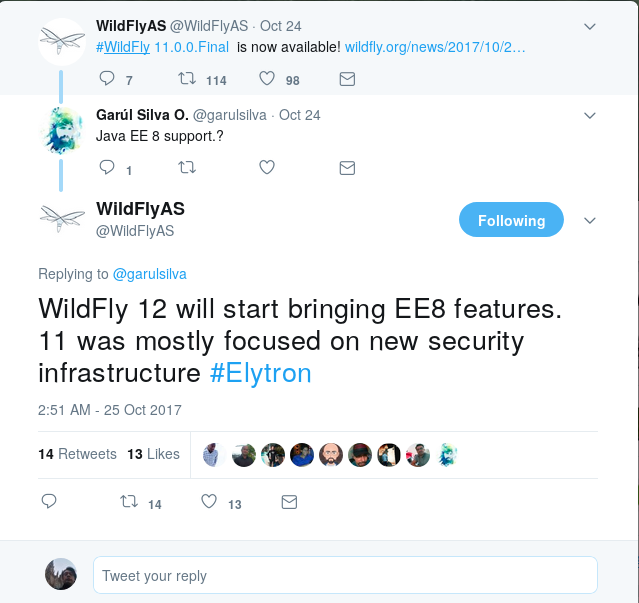
\includegraphics[width=0.7\linewidth]{Images/wildflyee8}
\end{figure}
\end{frame}


\begin{frame}{JavaEE 8}
\begin{figure}
\centering
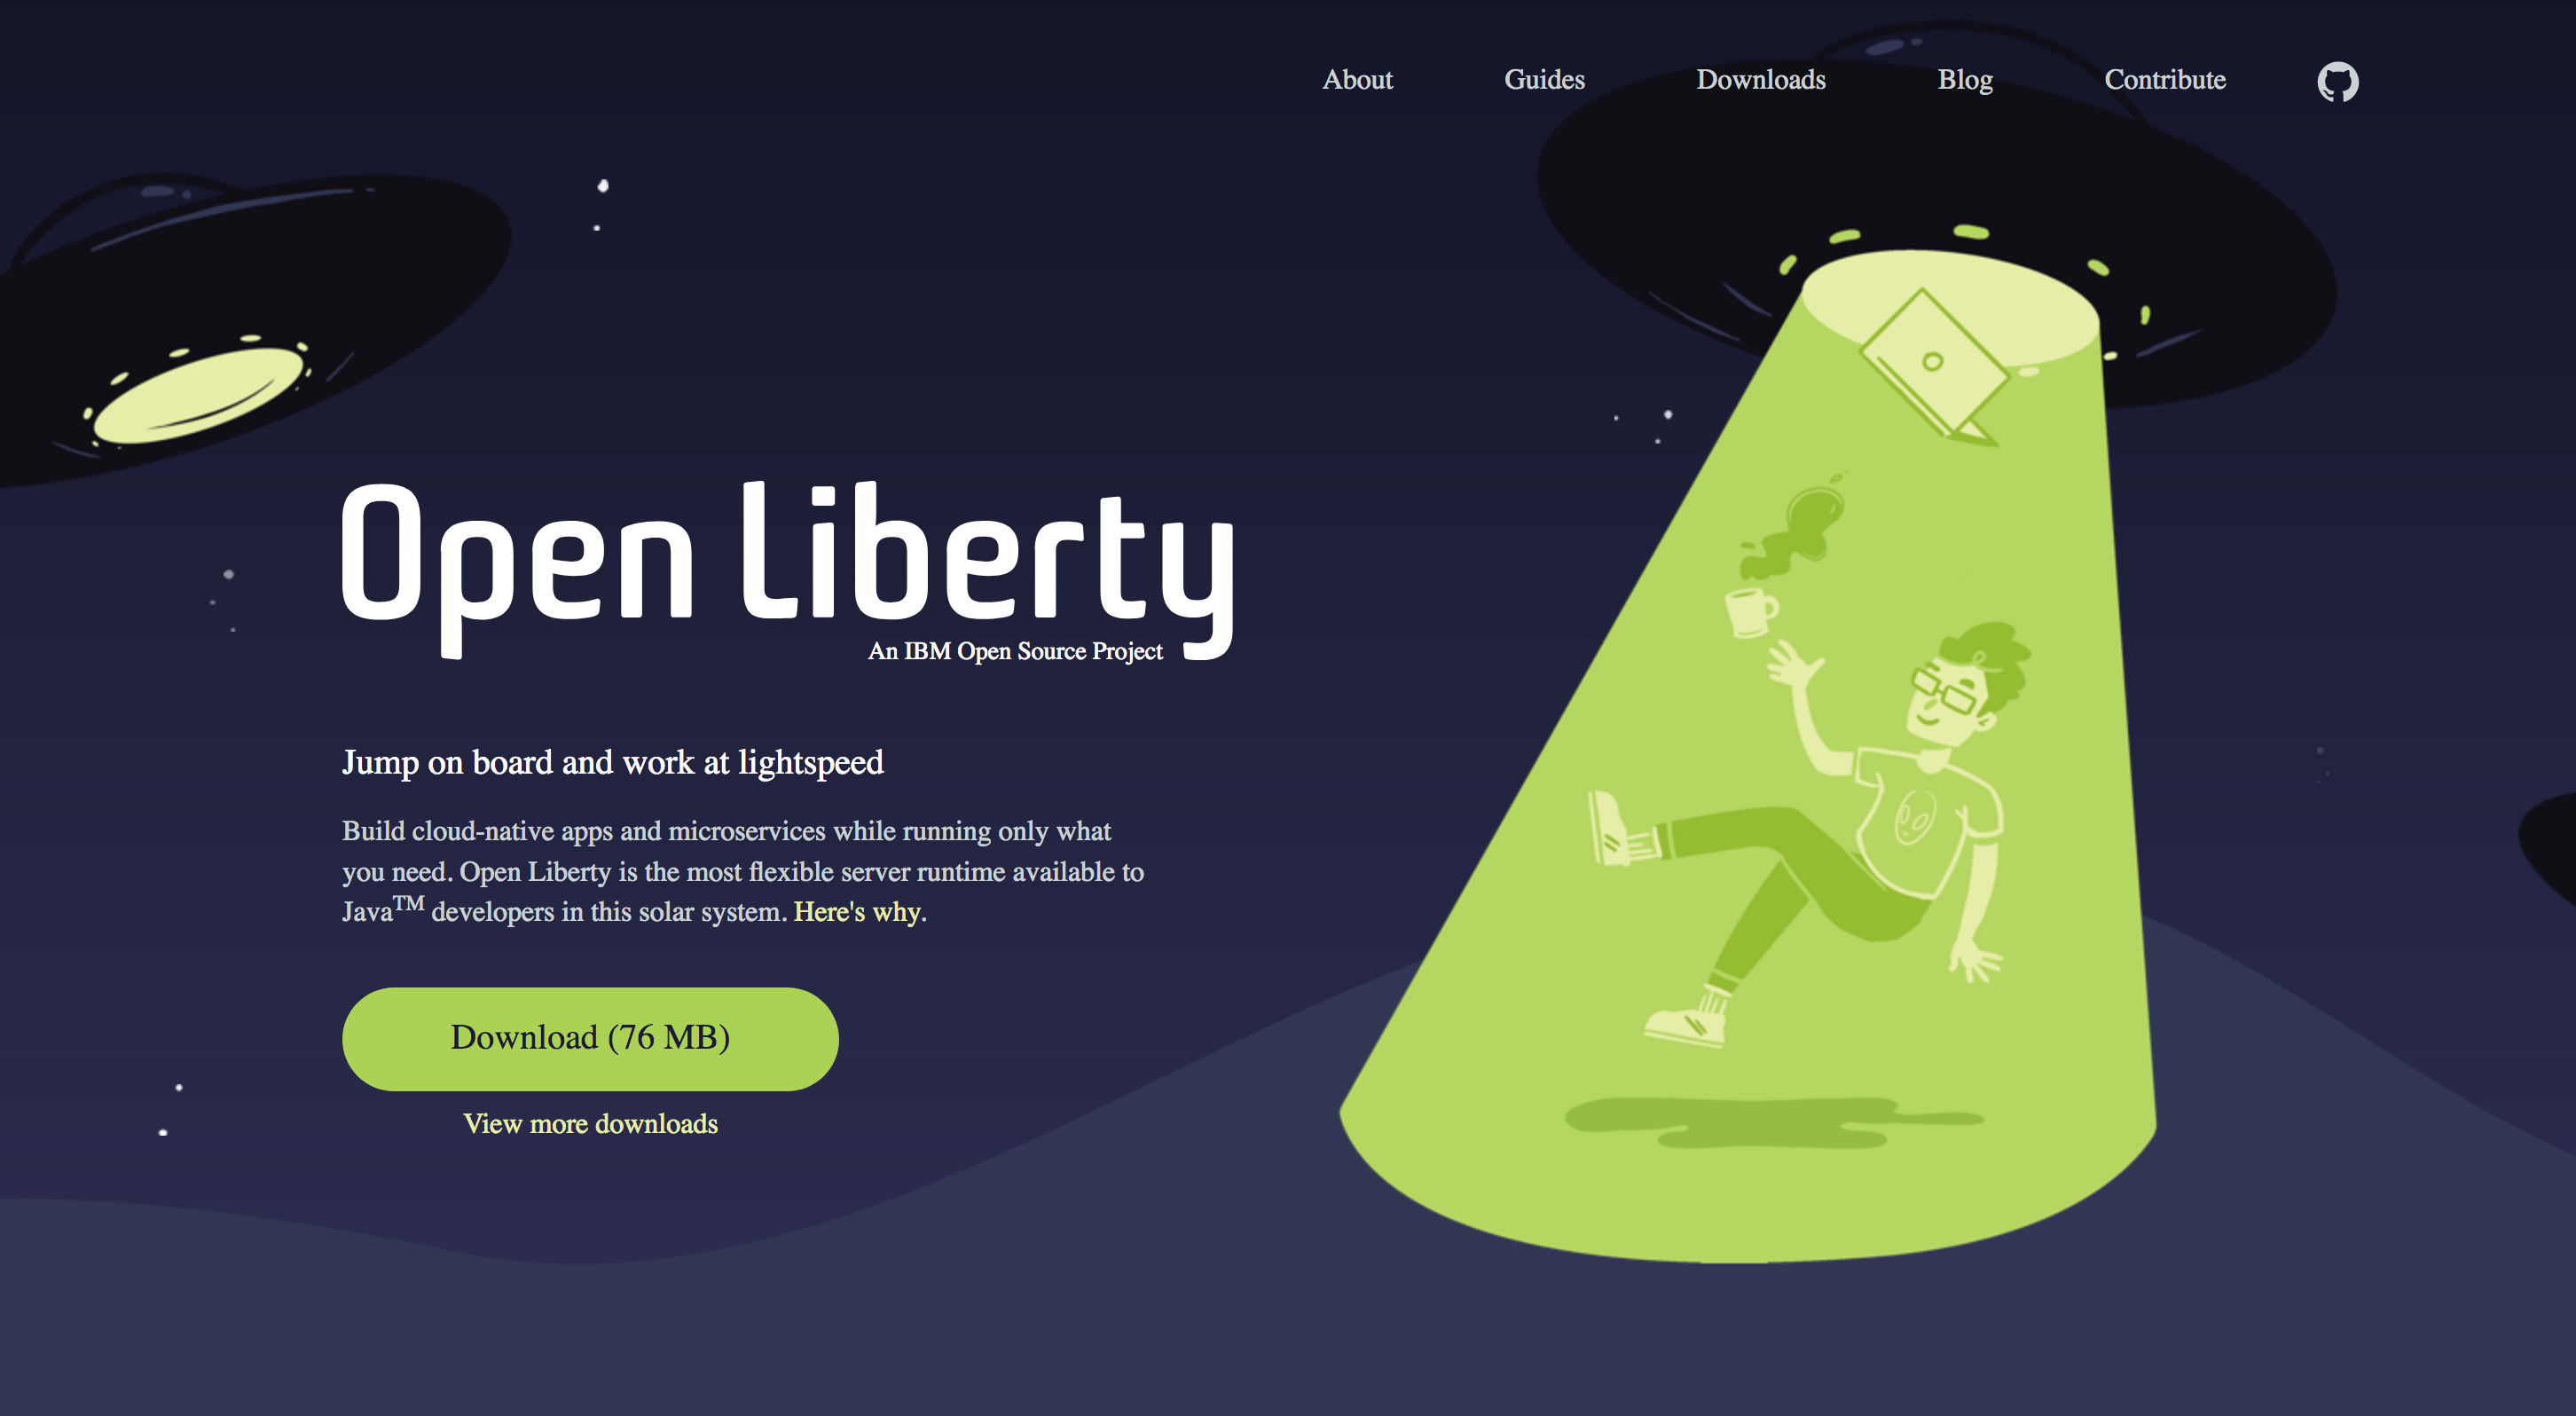
\includegraphics[width=\linewidth]{Images/liberty}
\end{figure}
\end{frame}

\begin{frame}{JavaEE 8}
\begin{itemize}
\item Glassfish – 100\% compatible con JavaEE 8
\item Wildfly(JBoss) – Inician los trabajos para JavaEE 8, se esperan para Wildfly 12
\item OpenLiberty – Fase beta de soporte
\item Payara – Fase beta de soporte
\item TomEE – Inican los trabajos para JavaEE 8
\item Weblogic – Compromiso publico que JavaEE 8 sera implementado
\end{itemize}
\end{frame}



\section{EE4J}


\begin{frame}{EE4J}
\begin{figure}
	\centering
	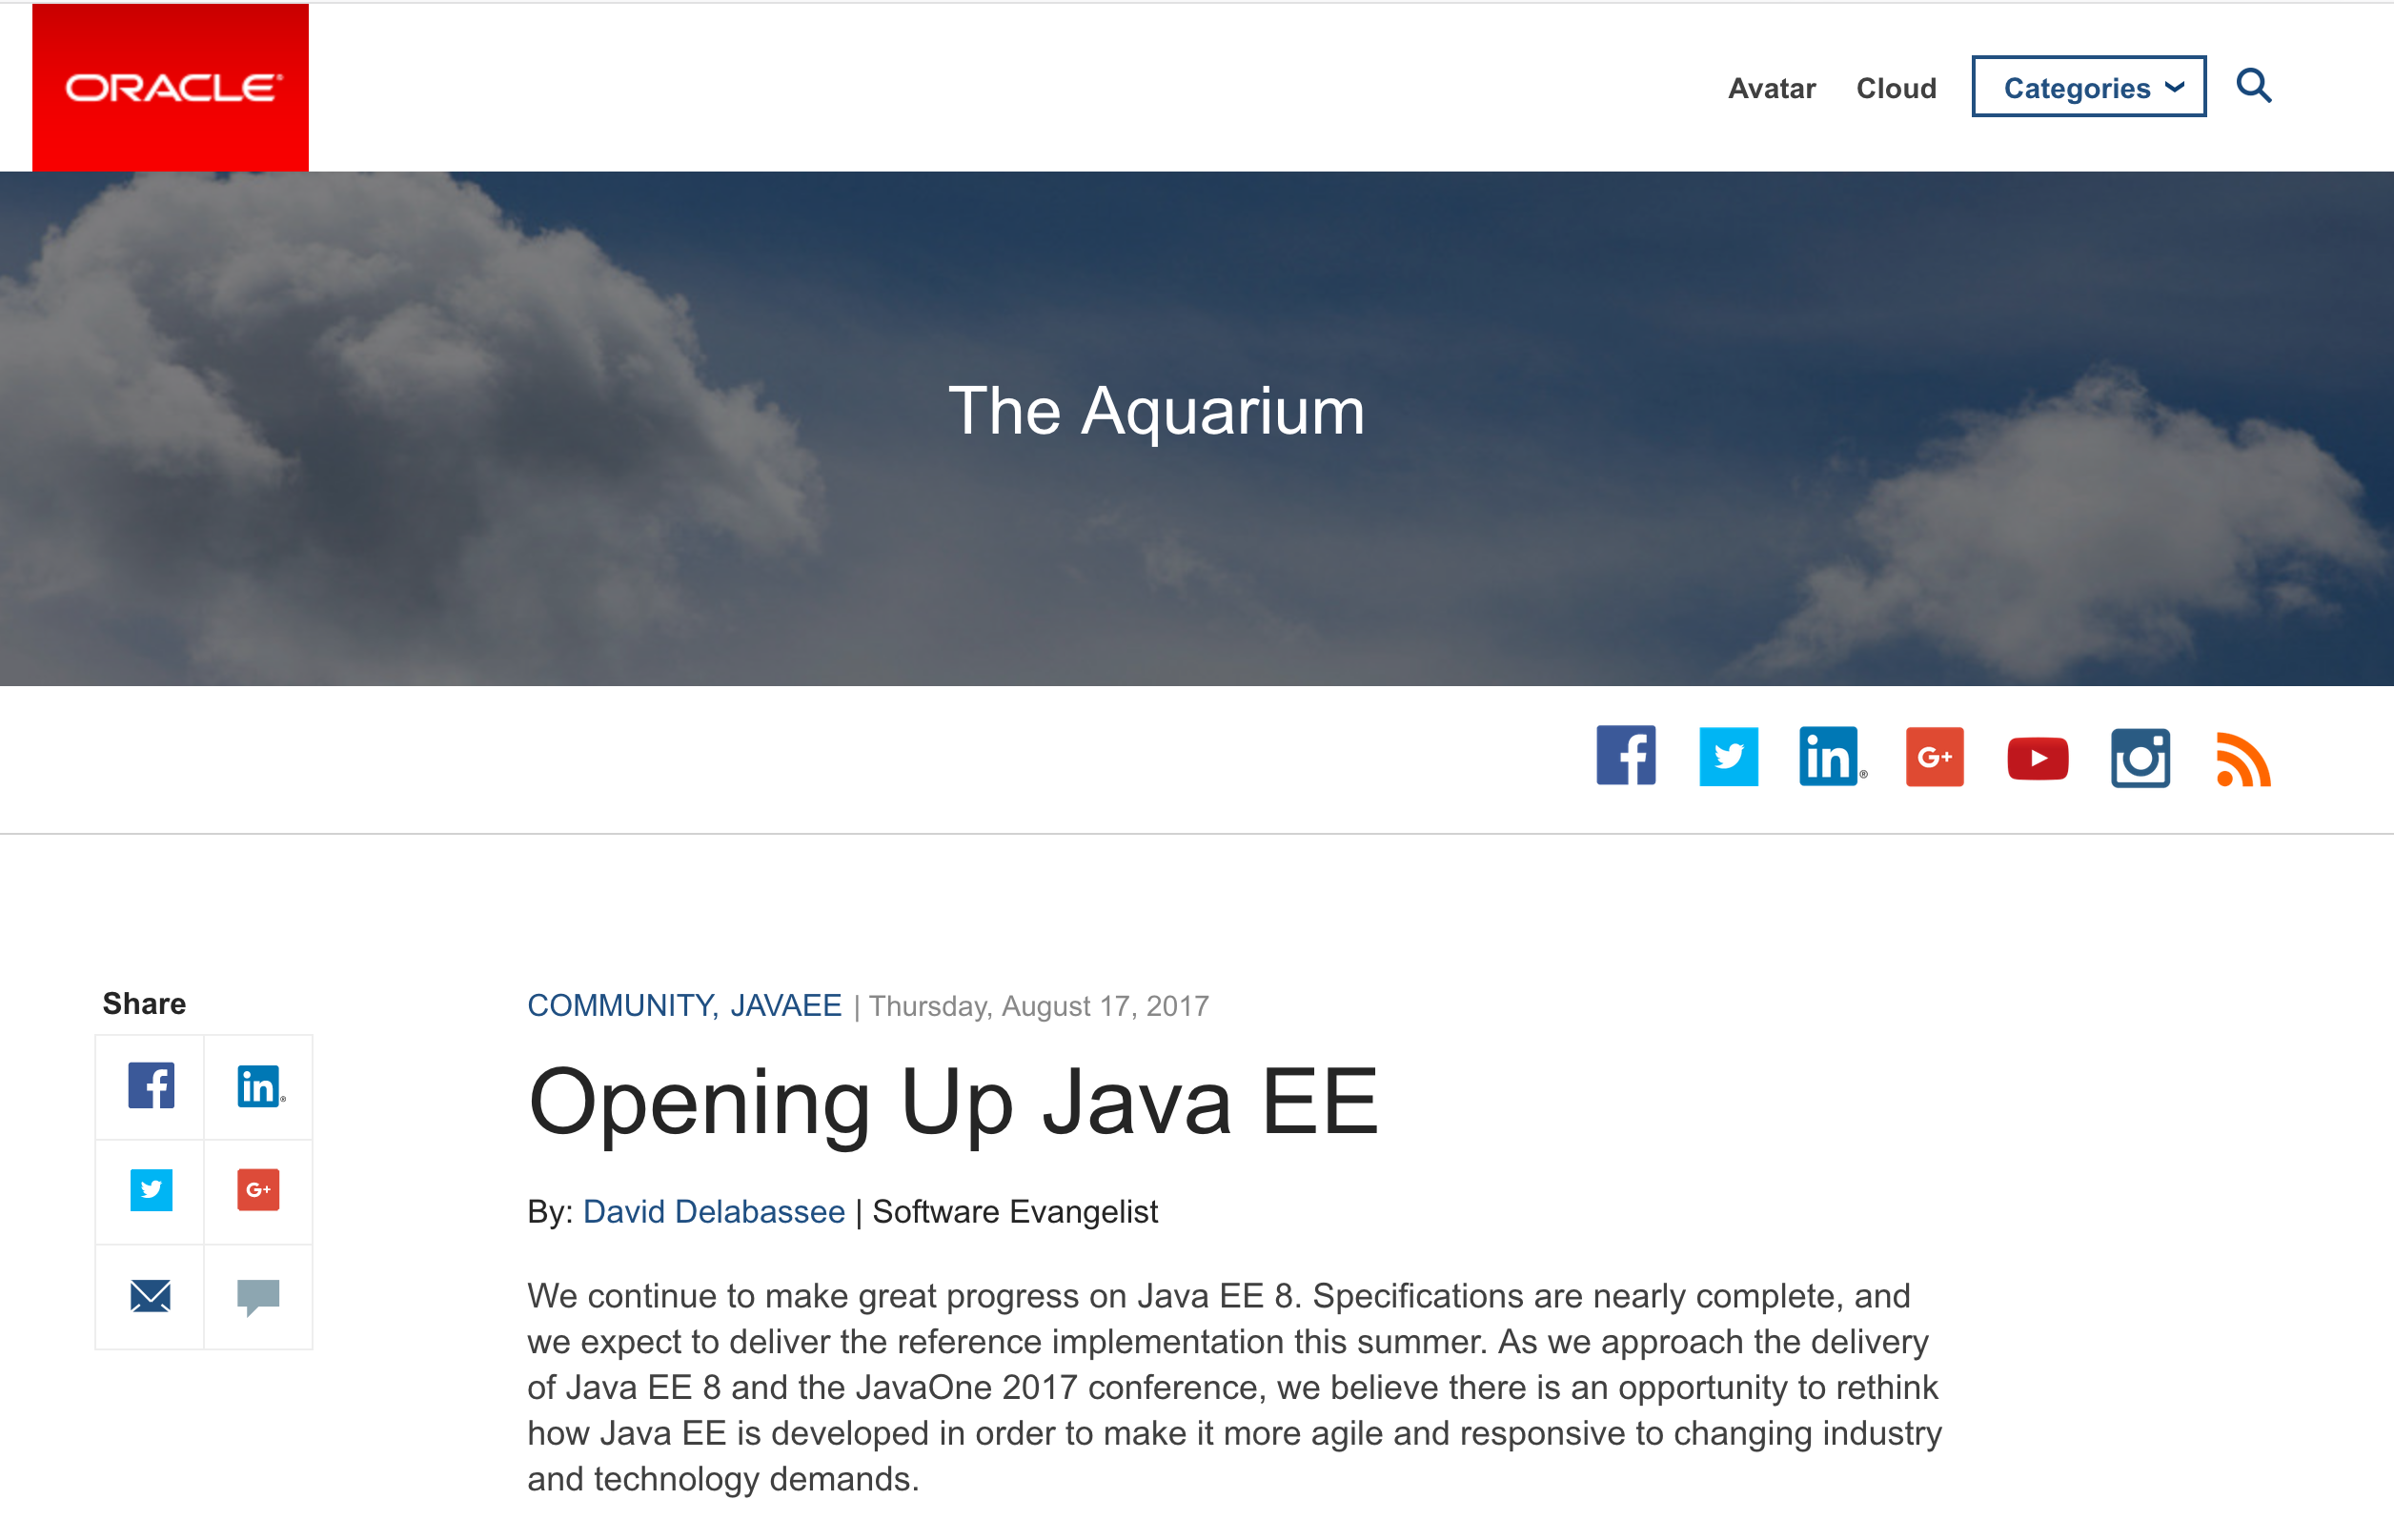
\includegraphics[width=\linewidth]{Images/javaeeopen}
\end{figure}
\end{frame}

\begin{frame}{EE4J}
\begin{figure}
	\centering
	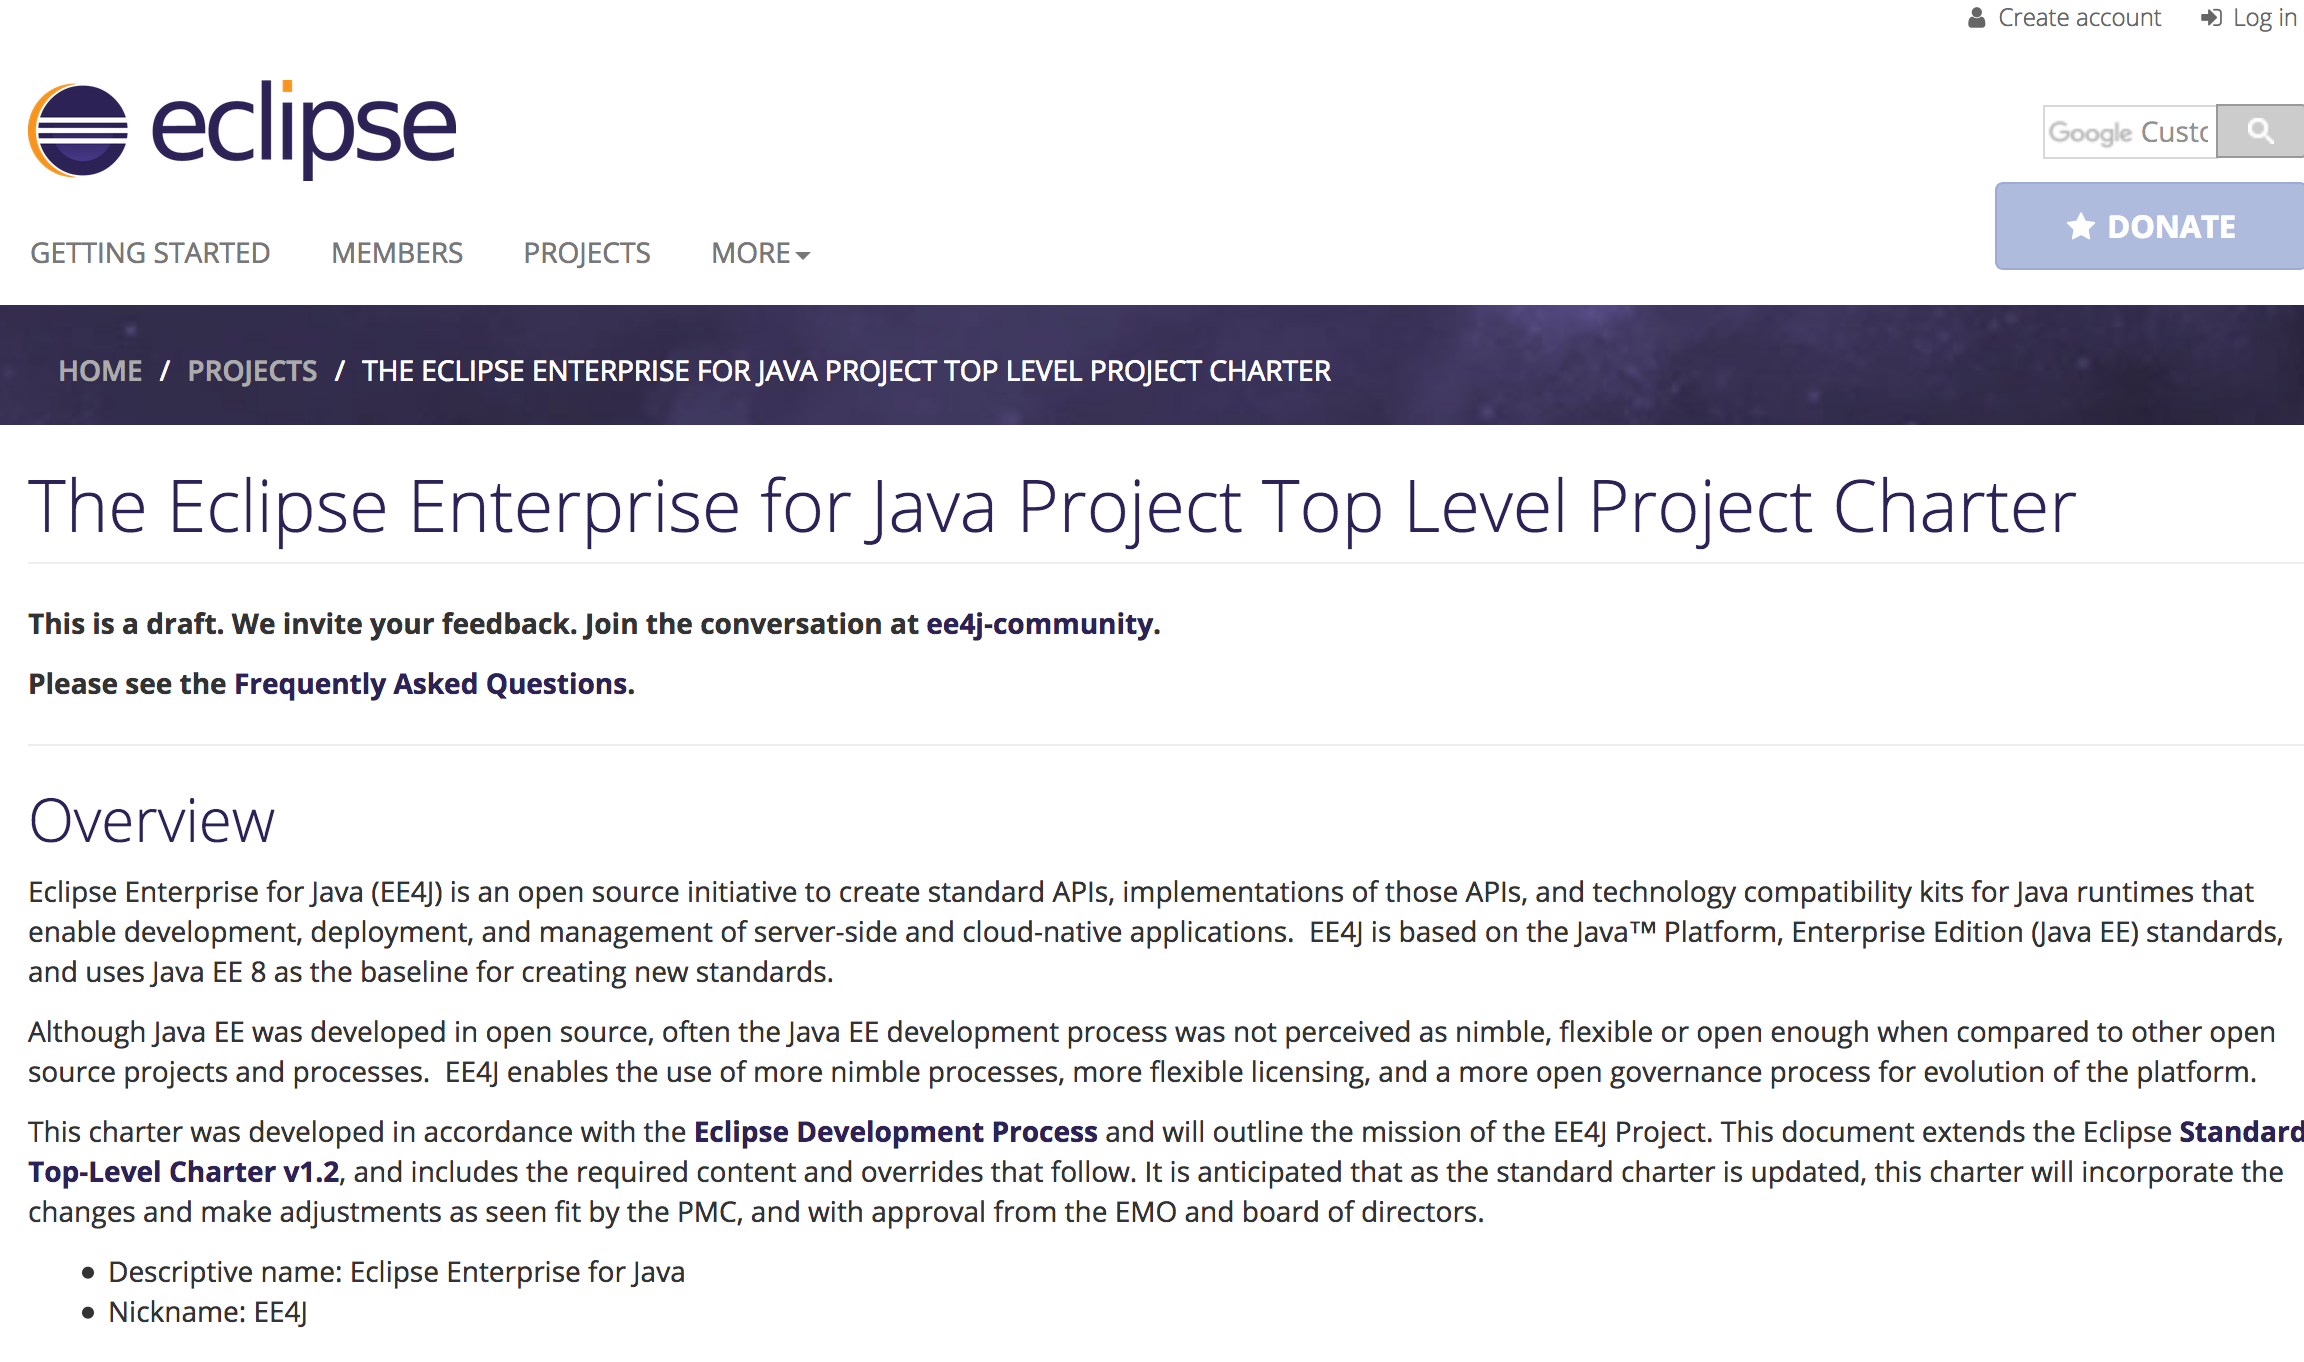
\includegraphics[width=\linewidth]{Images/ee4j}
\end{figure}
\end{frame}


\section{Fin}
\begin{frame}{Gracias}
\begin{itemize}
\item me@vorozco.com
\item http://vorozco.com
\item http://github.com/tuxtor/slides
\end{itemize}
\begin{center}

\includegraphics[width=0.1\linewidth]{Images/cclogo}
\\
This work is licensed under a Creative Commons Attribution-ShareAlike 3.0 Guatemala License.
\end{center}
\end{frame}
\end{document}

